\documentclass{beamer}

%% \documentclass[handout]{beamer}
%% % use this with the [handout] option to create handouts for the audience
%% \usepackage{pgfpages}
%% \pgfpagesuselayout{2 on 1}[a4paper,border shrink=5mm]

\mode<presentation>
{
  \usetheme{Diku}
% set this to your preferences:
%  \setbeamercovered{invisible}
  \setbeamercovered{transparent}
}

\usepackage{graphicx}
\usepackage{epic}

\usepackage{amsmath}
\usepackage{amssymb}
\usepackage{amsthm}

\newcommand{\basetop}[1]{\vtop{\vskip-1ex\hbox{#1}}}
\newcommand{\source}[1]{\let\thefootnote\relax\footnotetext{\scriptsize\textcolor{kugray1}{Source: #1}}}

% for coloured code citation in text:
\usepackage{fancyvrb}

%%%%%%%%%%%%%%%%%%%%%%%%%%%%%%%%%
%%%%%    code sections   %%%%%%%%
%%%%%%%%%%%%%%%%%%%%%%%%%%%%%%%%%

% code highlighting commands in own block
\DefineVerbatimEnvironment{code}{Verbatim}{fontsize=\scriptsize}
\DefineVerbatimEnvironment{icode}{Verbatim}{fontsize=\scriptsize}

% Fancy code with color commands:
\DefineVerbatimEnvironment{colorcode}%
        {Verbatim}{fontsize=\scriptsize,commandchars=\\\{\}}

%%%%%%%%%%%%%%%%%%%%%%%%%%%%%%%%%%
%%%%%    some coloring    %%%%%%%%

% use "DIKU green" from our color theme for \emph
\renewcommand{\emph}[1]{\textcolor{structure}{#1}}
% use some not-too-bright red for an \emp command
\definecolor{DikuRed}{RGB}{130,50,32}
\newcommand{\emp}[1]{\textcolor{DikuRed}{ #1}}
\definecolor{CosGreen}{RGB}{10,100,70}
\newcommand{\emphh}[1]{\textcolor{CosGreen}{ #1}}
\definecolor{CosBlue}{RGB}{55,111,122}
\newcommand{\emphb}[1]{\textcolor{CosBlue}{ #1}}
\definecolor{CosRed}{RGB}{253,1,1}
\newcommand{\empr}[1]{\textcolor{CosRed}{ #1}}

\newcommand{\mymath}[1]{$ #1 $}
\newcommand{\myindx}[1]{_{#1}}
\newcommand{\myindu}[1]{^{#1}}


%%%%%%%%%%%%%%%%%%%%

\title[Financial Software on GPUs]{GPGPU Programming Between \\ Neurodegenerative Disorders and \\ Finance}

\author[C.Andreetta/C.Oancea]{Christian Andreetta and  \emp{Cosmin Oancea}\\\texttt{christian.andreetta@diku.dk and \emp{cosmin.oancea@diku.dk}}}
\institute{HIPERFIT, Department of Computer Science\\University of Copenhagen}

\date[29.08.12 - \textsc{HIPERFIT}]{29.08.12 -- Science and IT Presentation}

\begin{document}

% \titleslide command WRAPS THIS SEQUENCE
%% % Set background to front page
%% \usebackgroundtemplate{\includegraphics[width=\paperwidth,height=\paperheight]{front}}
%% {
%% \begin{frame}[plain]
%%   \titlepage
%% \end{frame}
%% }
\titleslide

%%%%%%%% real content starts here %%%%%%%%%%

\begin{frame}
  \frametitle{Motivation}
  

{\sc gpgpu}: general-purpose graphics processing units \bigskip

Powerful Graphical Cards ({\sc gpgpu}s) are fundamental to gaming ...

\center \includegraphics[height=30ex]{figures/tank}  %\pause %\bigskip

\end{frame}


\begin{frame}
  \frametitle{Motivation}
  %\centering
\bigskip
... and ({\sc gpgpu}s) have also been used in other areas of less impact: \bigskip 

weather prediction, 
$\mbox{ }\mbox{ }\mbox{ }\mbox{ }\mbox{ }\mbox{ }\mbox{ }\mbox{ }\mbox{ }\mbox{ }\mbox{ }\mbox{ }\mbox{ }\mbox{ }\mbox{ }\mbox{ }$ 
$\mbox{ }\mbox{ }\mbox{ }\mbox{ }\mbox{ }\mbox{ }\mbox{ }$
bioinformatics,

\begin{center} 
\includegraphics[height=15ex]{figures/meteo}  
$\mbox{ }\mbox{ }\mbox{ }\mbox{ }\mbox{ }\mbox{ }\mbox{ }\mbox{ }\mbox{ }\mbox{ }\mbox{ }\mbox{ }\mbox{ }\mbox{ }\mbox{ }\mbox{ }$ 
\includegraphics[height=15ex]{figures/molecular_sim.jpg}  
\end{center} 
\smallskip

fluid-dynamic simulations,
$\mbox{ }\mbox{ }\mbox{ }\mbox{ }\mbox{ }\mbox{ }\mbox{ }\mbox{ }\mbox{ }\mbox{ }\mbox{ }\mbox{ }\mbox{ }\mbox{ }\mbox{ }\mbox{ }$ 
finance

\begin{center} 
\includegraphics[height=15ex]{figures/fluid_dyn_sim.png}  
$\mbox{ }\mbox{ }\mbox{ }\mbox{ }\mbox{ }\mbox{ }\mbox{ }\mbox{ }\mbox{ }\mbox{ }\mbox{ }\mbox{ }\mbox{ }\mbox{ }\mbox{ }\mbox{ }$ 
\includegraphics[height=15ex]{figures/finance.jpeg} 
\end{center}
\end{frame}


\begin{frame}
  \frametitle{Structure of the Presentation}
  \centering
 \begin{itemize} 
    \item Brief history of hardware: single-{\sc cpu}, multicores, {\sc gpgpu}. \smallskip

    \item Programming models for various hardware. \smallskip

    \item Hardware-independent language: map-reduce abstraction leads to inherently parallel programs. \smallskip

    \item In theory {\sc gpgpu} is superior to multicores; is this also the case in practice?
            Three real-world, big-compute applications on {\sc gpgpu}: \smallskip
    \begin{itemize}
        \item Structural Biology: modeling/understanding amyloid fibrillation \\ (insights in developing treatment for various illnesses) \smallskip
        \item Finance: pricing a financial contract (via Monte-Carlo iteration)  \smallskip %\\ (i.e., what is the value of a contract now?)
        \item Finance: understanding the market over which contracts are priced
    \end{itemize} \smallskip

    \item Evidence that compiler optimizations may match the efficiencies of hand-tuned {\sc gpgpu} code.
\end{itemize} 
\end{frame}


\begin{frame}
  \frametitle{Brief Hardware History} % of CPU, Multicores, GPGPU
  \centering
\begin{itemize}
    \item How did general-purpose graphics-processing units (\emph{{\sc gpgpu}}) come to being? \bigskip %\pause \bigskip
    
    \item In the beginning was the \emph{Single-CPU}, \smallskip \\ 
            and the \emph{single-CPU} was sequentially-programmable, \smallskip \\ 
            and sequential code was programming. \bigskip

    \item Then the frequency of the single-CPU could not be further increased and \emph{Multi-cores/processors} were born. \bigskip

    \item And ``Hardware Engineers'' worked hard to support the illusion that random-access to memory has uniform cost: \\ \smallskip
        \begin{itemize}
            \item   thrown many transistors to memory-hierarchy coherency and such\\ \smallskip
            \item   ... and ultimately (arguably) they have failed (to scale up)!
        \end{itemize} \bigskip
%\bigskip
%
%    \item But, but, but ... is the sequentially-written code going to benefit?
\end{itemize}
\end{frame}

\begin{frame}
  \frametitle{Brief Hardware History (Continuation)} % of CPU, Multicores, GPGPU
  \centering
 \begin{itemize}
    \item Then ``Hardware Engineers'' fixed \emph{scalability} with \emph{{\sc gpgpu}} but took away \emp{programming convenience}:  \smallskip
        \begin{itemize}
            \item single-instruction multiple-data ({\sc simd}): 
                \begin{itemize}
                    \item cannot make an omelet with one core and a steak with the next,
                    \item but you can make first an omelet, then a steak, both very fast. 
                \end{itemize}\smallskip
            \item non-uniform, explicitly programmable memory hierarchy. 
        \end{itemize}
\end{itemize}

\begin{center} 
\includegraphics[height=20ex]{figures/MulticoreArch.png}  
$\mbox{ }\mbox{ }\mbox{ }\mbox{ }\mbox{ }\mbox{ }\mbox{ }\mbox{ }\mbox{ }\mbox{ }\mbox{ }\mbox{ }\mbox{ }\mbox{ }\mbox{ }\mbox{ }$ 
\includegraphics[height=20ex]{figures/GPGPUarch.png}  
\end{center} 

\end{frame}

\begin{frame}
  \frametitle{Theoretical Hardware Comparison: CPU vs GPGPU} % of CPU, Multicores, GPGPU

{\sc gpgpu} shows superior peak bandwidth and compute power vs. {\sc cpu}.  \bigskip

$x_1 + x_2$: bring the values of $x_1$ and $x_2$ from memory than add the values together.


\begin{center} 
\includegraphics[height=27ex]{figures/Bandwidth.png}  
%$\mbox{ }$ 
\includegraphics[height=27ex]{figures/GFlops.png}
\end{center} 

\end{frame}


\begin{frame}
  \frametitle{Comparison: Sequential {\em vs} Parallel Code} % of CPU, Multicores, GPGPU

\begin{itemize}
    \item Writing sequential code: 
        buy 100 eggs \alert{then} buy 100 apples \alert{then} make an omelet \alert{then} make a pie \bigskip 

    \item Does parallel hardware benefit directly the sequential code? No! \smallskip
        Dependencies: can't make an omelet without breaking eggs! \bigskip
        
    \item Programming for multicores: \smallskip
            you buy 100 eggs and \emph{in parallel} your sister buys 100 apples \smallskip
            \alert{then} you make an omelet and \emph{in parallel} your sister makes a pie \bigskip
        
    \item Programming with {\sc gpgpu}: \smallskip \\
            each of 1000 people buys \emph{in parallel} 1 egg   (1000 eggs)   \alert{then} \\ 
            each of 1000 people makes \emph{in paralle} an 1-egg omelet \alert{then} \\
            the 1-egg omelets are put together $\Rightarrow$ 1000-egg omelet \alert{then} ... \bigskip


    \item Trouble is writing efficient (parallel) code for \emp{multicores} is not as easy
            as we would like and it gets much worse with \emp{{\sc gpgpu}s}.
\end{itemize}


\end{frame}


%\visible<2-4>{
%\includegraphics[scale=0.215]{Figures/PerfectResO2.pdf} } \includegraphics[scale=0.215]{Figures/Spec2006Res}
%\includegraphics[scale=0.215]{Figures/PerfectResO2.pdf}  \includegraphics[scale=0.215]{Figures/Spec2006Res}
%\includegraphics<2-4>[scale=0.215]{Figures/PerfectResO2.pdf}



\begin{frame}
  \frametitle{High-Level Perspective} % of CPU, Multicores, GPGPU
  \centering

\begin{itemize}

\item \emp{Language} should be hardware independent. \bigskip

\item \emp{Language} should preserve as much as possible algorithmic invariants (automatic optimization). \bigskip

\item {\em Consequence}: if the algorithm is inherently parallel than this should 
                        also be easily derivable from the implementation. \bigskip
%an inherently-parallel algorithm should have an easily derivable parallel implementation. 

\item Write-now, compile-and-run-in-twenty-years programs: 
    \begin{itemize} 
        \item the compiler is the depositary of the intelligence that 
                allows efficient execution (on various hardware).
    \end{itemize} \bigskip

\item What is the programming abstraction? \bigskip

\end{itemize} 

\end{frame}

\begin{frame}
  \frametitle{Programming Basic Blocks: Map-Reduce Style} % of CPU, Multicores, GPGPU


Example: \alert{map} (add 1) [1, 2,.., n]  $\rightarrow$ [2, 3, ..., n+1] \smallskip

In General: \alert{map} f [$a_1$, $a_2$, ..., $a_n$] $\rightarrow$ [f($a_1$), f($a_2$), ..., f($a_n$)] \bigskip



Example: \alert{reduce} (+) [1, 2, 3, 4, 5] $\rightarrow$ 1+2+3+4+5 = 15 \smallskip

In General: \alert{reduce} $\odot$ [$a_1$, $a_2$, ..., $a_n$] $\rightarrow$ $a_1 \odot a_2 \odot ... \odot a_n$ \bigskip



Requires $\odot$ to be an associative binary operator, i.e., $(a_1 \odot a_2) \odot a_3 = a_1 \odot (a_2 \odot a_3)$ \\ \smallskip

Example: addition, i.e., (1 + 2) + 3 = 1 + (2 + 3) = 6  \bigskip


\alert{map} is inherently parallel. How about \alert{reduce}?


\end{frame}


\begin{frame}
  \frametitle{Computing Reduce in Parallel}

\begin{center} 
        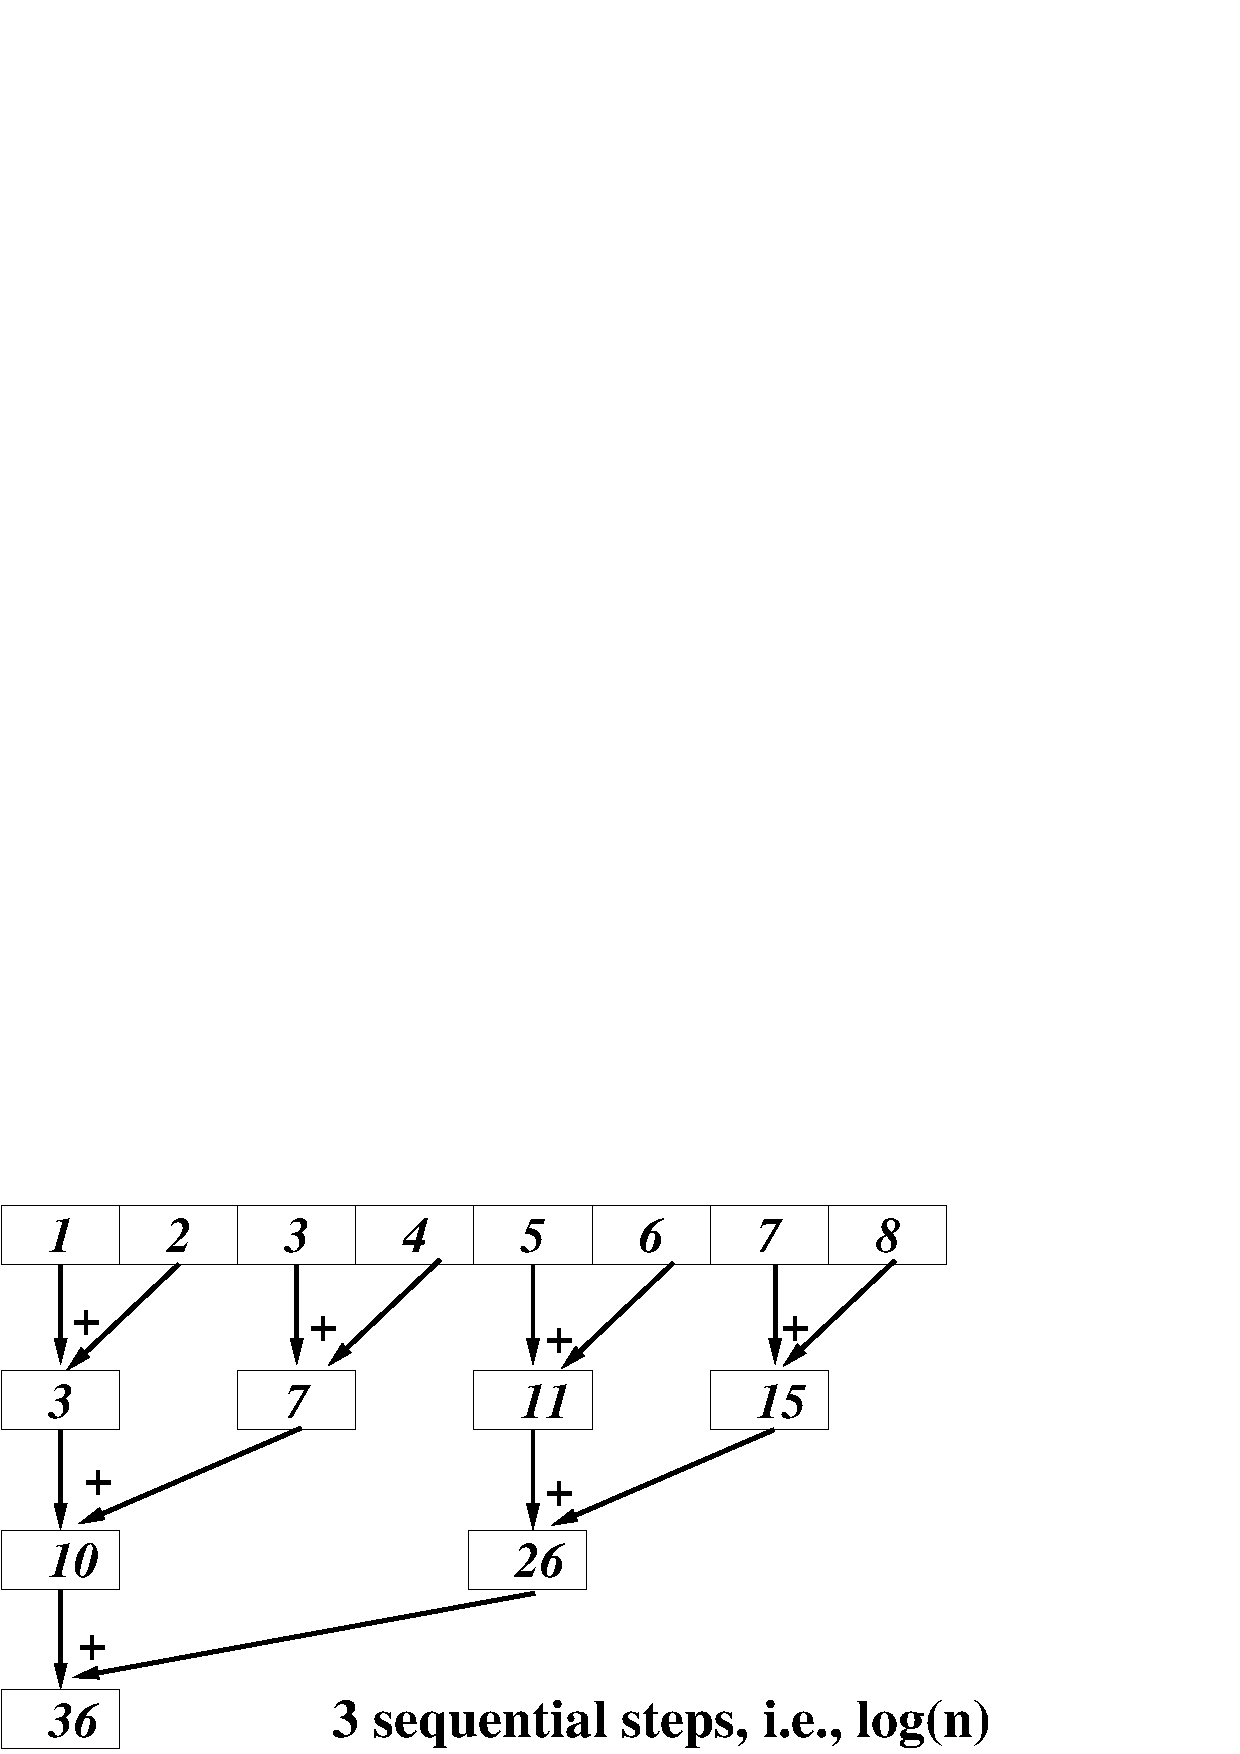
\includegraphics[height=28ex]{figures/ReduceEg.pdf} 
\end{center} 

We build programs by combining \alert{map} and \alert{reduce}. Example: \smallskip

\emp{scan} (+) [1, 2, 3, 4] $\rightarrow$ [1, 1+2, 1+2+3, 1+2+3+4] $\rightarrow$ [1, 3, 6, 10]\bigskip

And next we look at some real-world programs:
\end{frame}

%Amyloid fibrillation: an important class of human diseases
%	amyloid: waxy translucent substance, typically protein-based
%	fibrillation: etymology related to fibers, and irregularity

\begin{frame}
  \frametitle{Structural Biology Case Study}
\bigskip
    {\em \emp{Amyloid fibrillation}} is the process of formation of fiber in biological tissues; this affects negatively cell-to-cell communication.

\bigskip

    The Figure shows an amyloid formation in brain tissue:

    \begin{center} 
        \includegraphics[height=30ex]{figures/AmyloidBrain.png} 
    \end{center} 
 
\end{frame}

\begin{frame}
  \frametitle{Structural Biology Case Study (Continuation)}
\bigskip
    {\em \emp{Amyloid fibrillation}} is the process of formation of fiber in biological tissues; this affects negatively cell-to-cell communication.

\bigskip

The Figure on the right depicts (Parkinson) protein mis-aggregation. %that causes amyloid fibrillation. 

\begin{center} 
    \includegraphics[height=30ex]{figures/AmyloidDiseases.png} 
$\mbox{ }\mbox{ }\mbox{ }\mbox{ }\mbox{ }\mbox{ }\mbox{ }\mbox{ }\mbox{ }\mbox{ }\mbox{ }$
    \includegraphics[height=30ex]{figures/Amyloid2.jpg} 
\end{center} 
 
\end{frame}

\begin{frame}
  \frametitle{Structural Biology Case Study (Continuation)}
\bigskip
%    The task is to model the protein mis-aggregation 
    Small Angle X-ray/Neutron Scattering ({\sc saxs}):  \\
        provides aggregate data (3d $\rightarrow$ 1d) with low resolution properties.


\begin{center} 
    \includegraphics[height=30ex]{figures/SAXSprocess.jpg} 
\end{center} 

    Task: we have the output ({\sc saxs}) and need to find its corresponding protein structure.
        	An inverse problem!
\end{frame}

%Ill-conditioned and ill-posed problem:
%	solution: Monte Carlo simulations
%
%		proposals: biologically reasonable structures
%		evaluation: forward computation of the theoretical Scattering curve
%		exploration: acceptance/rejection based on the similarity between
%						proposal and experimental Scattering

\begin{frame}
  \frametitle{Structural-Biology Case-Study Speedup}

%    The task is to model the protein mis-aggregation 
    The inverse problem is solved via Monte Carlo simulations: \smallskip
\begin{itemize}
    \item \emph{proposals}: biologically reasonable structures, \smallskip
    \item \emph{evaluation}: computation of the theoretical Scattering curve, \smallskip
    \item \emph{exploration}: acceptance/rejection based on the similarity between 
						proposal and experimental Scattering. \smallskip
\end{itemize}


\begin{center} 
    \includegraphics[height=11ex]{figures/ProteinStructIncomplete.png} 
$\mbox{ }\mbox{ }\mbox{ }\mbox{ }\mbox{ }\mbox{ }$
    \includegraphics[height=12ex]{figures/ProteinStructFinal.png} 
\end{center} 

Before the simulation (left) the middle-part structure was unknown. \smallskip

The information recovered via Monte-Carlo simulation (right) is crucial for designing 
drug targets to treat the disease.

%\begin{center} 
%    \includegraphics[height=24ex]{figures/AmyloidSpeedup.png} 
%\end{center} 
%
%Speedup on GTX 580 vs the sequential {\sc cpu} execution. The $X$ axis represents the number of distinct amino-acids of the protein.

\end{frame}

\begin{frame}
  \frametitle{Structural-Biology: GPGPU-CPU Comparison}

Speedup on GTX 480 {\em vs} seq. {\sc cpu} execution. HIGHER is BETTER!\\ $X$ axis: the number of distinct amino-acids of the protein.


%    The task is to model the protein mis-aggregation 

\begin{center} 
    \includegraphics[height=24ex]{figures/AmyloidSpeedup.png} 
\end{center} 

{\em \emp{Equivalent of $20$ ideal-multicore machines, each with $16$ cores!}}

%Assuming a top-end machine with $16$ multicores, and ideal speedup (i.e., $16\times$) 
%   we would need about $20$ such machines to match the result of one gaming {\sc gpgpu}! 

\end{frame}

\begin{frame}[fragile,t]
\frametitle{Finance: Pricing a Contract Problem Statement}

{\em \emph{Contract Example}}: \emp{Receive} $1000$ DKK on Dec. $24^{th} 2012$, and \emp{Return} in one year 
                    time $900$ DKK plus the summed difference between stocks $X$ and 
                    $Y$ measured at dates March $1^{st}$, May $1^{st}$ and Dec. $1^{st} \mbox{ }2013$. 

\bigskip

I receive an offer to buy this contract today for $100$ DKK. 

\bigskip

\emph{Should I?} % How do I compute what is the value of this contract today?

\bigskip

\begin{center}
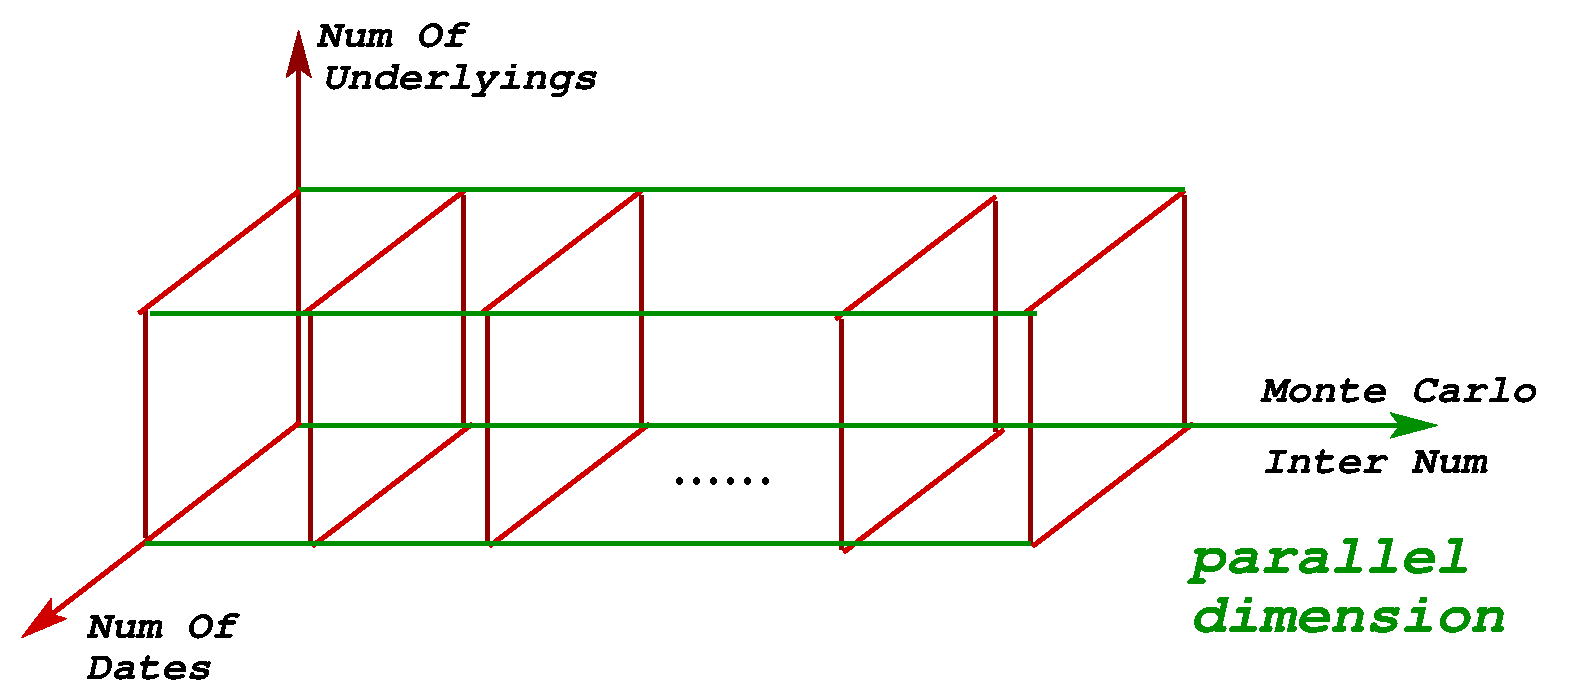
\includegraphics[height=20ex]{Figures/PricingMemSpace}
\end{center}

\end{frame}


\begin{frame}[fragile,t]
\frametitle{Finance: Pricing a Contract on GPGPU}

Speedup on mobile and gaming {\sc gpgpu}s {\em vs} sequential {\sc cpu} execution. HIGHER is BETTER!
\smallskip
\begin{center} 
\includegraphics[height=26.5ex]{figures/optimizations-GPU-CG-1.png} 
$\mbox{ }\mbox{ }\mbox{ }\mbox{ }$
\includegraphics[height=26.5ex]{figures/optimizations-GPU-CG-0.png} 
\end{center} 
\smallskip
{\em \emp{In an ideal-{\sc cpu} world, matching the average speedup requires\\ a $44$-multicore laptop and \\ a $317$-multicore desktop!}}

\end{frame}

\begin{frame}[fragile,t]
\frametitle{Finance: Modeling the Market}

\bigskip

Compute function $f(x,t)$, $f : \mathcal{S} \times [0, T] \rightarrow \mathbb{R}$, 
which solves the second order partial differential equation:

\bigskip

\begin{equation}
\frac{\partial f}{\partial t}(x,t)\mbox{ }+\mbox{ }\mu(x,t)\frac{\partial f}{\partial x}(x,t)\mbox{ }+\mbox{ }
\frac{1}{2}\sigma(x,t)^{2}\frac{\partial^{2} f}{\partial x^{2}}(x,t)\mbox{ }-\mbox{ }
r(x,t)f(x,t) = 0
\end{equation}

\bigskip

with terminal condition $f(x, T) = F(x), x \in \mathcal{S}$, where $F$ is known.

\bigskip
\bigskip
\bigskip

\emp{It comes down to solving this equation for many instances of $\mu, \sigma, r$.}


\end{frame}


\begin{frame}[fragile,t]
\frametitle{Finance: Modeling the Market on GPGPU}

\smallskip
\begin{center} 
\includegraphics[height=26.5ex]{figures/CrankNicGPU.pdf} 
\end{center} 
\smallskip

Well, in this case the multicore {\sc cpu} might have a chance to catch up.

\end{frame}

\begin{frame}[fragile,t]
\frametitle{Finance: Modeling the Market on multicore CPU}

\smallskip
\begin{center} 
\includegraphics[height=26.5ex]{figures/CrankNicCPU.pdf} 
\end{center} 
\smallskip

No, it does not catch up due to limited bandwidth!

\bigskip

\emph{So the theoretical comparison between {\sc gpgpu} and multicore-{\sc cpu} architectures seems to also hold in practice!}

\end{frame}


\begin{frame}
  \frametitle{Programming on GPGPU}

\begin{itemize}
    \item Why is it that {\sc gpgpu} programming is not mainstream? \bigskip %\pause 

    \item Hint: we have shown wonderful speedups, \\ but not a word about the pain (think programming in assembly)  \bigskip %\pause 

    \item Because {\sc gpgpu} hardware is more difficult to program: \smallskip
        \begin{itemize}
            \item the memory hierarchy is not transparent to the user anymore, \smallskip
            \item irregular memory accesses incur high-overheads,              \smallskip
            \item limited tools: debugging is a nightmare.                     \bigskip    %\pause
        \end{itemize}  

    \item Because the optimization strategies for {\sc gpgpu} and {\sc cpu} differ. \bigskip %\pause 

    \item Because not all programs are suitable to be run on {\sc gpgpu}.
\end{itemize}

\end{frame}

\begin{frame}
  \frametitle{How to Make GPGPU Mainstream?}

\begin{itemize}
    \item Hardware-independent language with good support for (mathematical) abstraction. \bigskip %\pause 

    \item Compiler: exploits algorithmic invariants to best suit the hardware platform.  \bigskip %\pause 

    \item Seems doable: we give two example of simple optimizations that show good impact.
\end{itemize}

\end{frame}




\begin{frame}[fragile,t]
  \frametitle{Impact of Memory-Coalescing Optimization}

Speedup on mobile and gaming {\sc gpgpu}s with memory-coalescing \\ 
optimization \empr{ON} (red) and \emphb{OFF} (blue). HIGHER is BETTER!
\smallskip
\begin{center} 
\includegraphics[height=25.5ex]{figures/optimizations-GPU-MC-1.png} 
$\mbox{ }\mbox{ }\mbox{ }\mbox{ }$
\includegraphics[height=25.5ex]{figures/optimizations-GPU-MC-0.png} 
\end{center} 
\smallskip

\emp{Not natural but effective transformation, hence suited to be implemented in the repertoire of an optimizing compiler.}

\end{frame}





\begin{frame}[fragile,t]
  \frametitle{Impact of Map Fusion/Distribution}

Speedup on mobile and gaming {\sc gpgpu}s with map fusion \\ 
\emphb{ON} (blue) and map distribution \empr{ON} (red). HIGHER is BETTER!
\smallskip
\begin{center} 
\includegraphics[height=25.5ex]{figures/optimizations-GPU-CG-1.png} 
$\mbox{ }\mbox{ }\mbox{ }\mbox{ }$
\includegraphics[height=25.5ex]{figures/optimizations-GPU-CG-0.png} 
\end{center} 
\smallskip

Impact is input-sensitive; but a cost model can chose at runtime the better alternative.

\end{frame}


\begin{frame}
  \frametitle{Conclusions}

\begin{itemize}
    \item Shown several killer applications for {\sc gpgpu}. \bigskip
    \item Hardware-independent language with good-abstraction level + powerful compiler optimizations \smallskip  %$Rightarrow$ {\sc gpgpu} becomes mainstream \smallskip
        \begin{itemize}
            \item because we want to keep algorithm's implementation clean, \smallskip
            \item because optimizations are hardware dependent and hardware changes, \smallskip
            \item because the optimization space is rich and data-sensitive. \bigskip
        \end{itemize}
    \item Identified several compiler optimizations that have the potential to match 
            the efficiency of hand-tuned {\sc gpgpu} code.  
\end{itemize}
\end{frame}

%%%%%%%%%%%%%%%%%%%%%%%%%%%%%%%%%%%%%%%%%
%%% It ends here!
%%%%%%%%%%%%%%%%%%%%%%%%%%%%%%%%%%%%%%%%%


\end{document}

